% small.tex
\documentclass{beamer}
\usetheme{Boadilla}

\setbeamertemplate{author in head/foot}{\insertshortauthor}
\setbeamertemplate{navigation symbols}{}
\setbeamertemplate{caption}{\raggedright\insertcaption\par}

\begin{document}

\title[HPC]
{High Performance Computing}
\author[smithc11@rpi.edu]{Cameron W. Smith}
\institute[SCOREC]{
Computational Scientist \\
Ph.D Candidate, Computer Science \\
\smallskip
Scientific Computation Research Center \\
Center for Computational Innovations \\
Rensselaer Polytechnic Institute
}

%----------- titlepage ----------------------------------------------%
\begin{frame}[plain]
  \titlepage
\end{frame}

\begin{frame}
  \frametitle{What is computed?}
  \center All the things.
  \begin{figure} \centering
    
\includegraphics[width=.8\textwidth]{figs/plainDogeZoom.png}
    %http://barkpost-assets.s3.amazonaws.com/wp-content/uploads/2013/11/plainDoge.jpg
  \end{figure}
\end{frame}

\begin{frame}
  \frametitle{Why?}
  \center It's cheaper.
  \center It's easier.
  \center It's faster.
\end{frame}

\begin{frame}
  \frametitle{Where?}
  \center At RPI.
  \center At other universities.
  \center At national laboratories.
  \center At businesses.
  \center At undisclosed locations operated by government agencies...
\end{frame}

\begin{frame}
  \frametitle{Who?}
  \center Engineers
  \center Biologists
  \center Chemists
  \center Physicists
  \center Cryptologists
  \center Computer Scientists
  \center Quantitative Analyst
  \center Astronomers
  \center Doctors
\end{frame}

\begin{frame}
  \center Everyone.
\end{frame}

\begin{frame}
  \frametitle{Aerospace Engineers}
  \begin{figure} \centering
    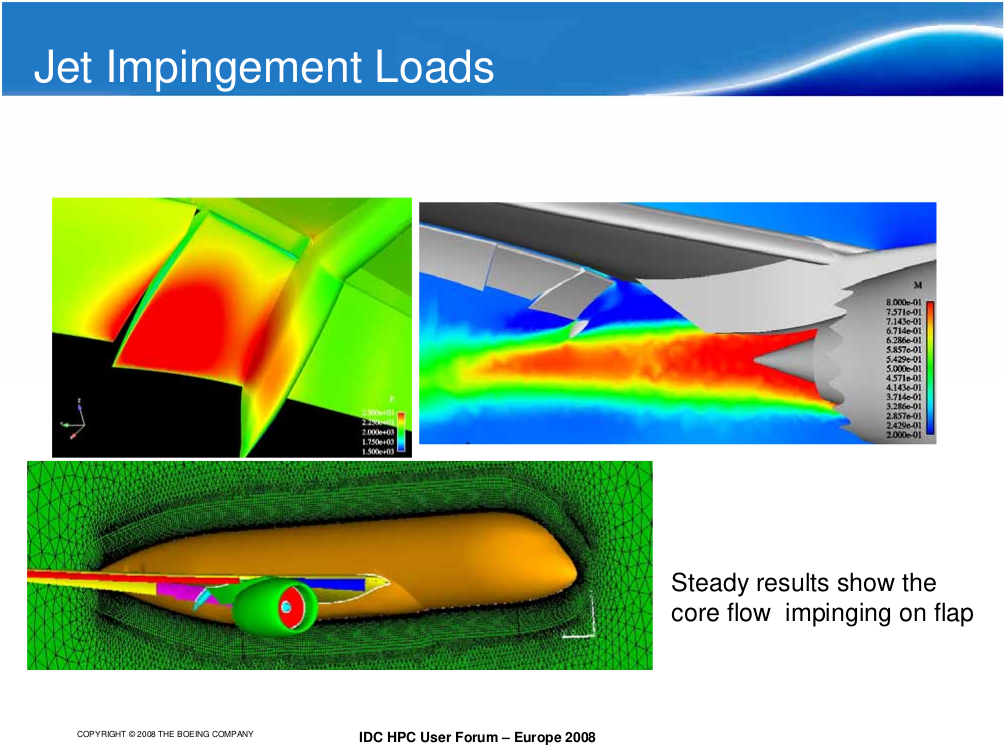
\includegraphics[width=.8\textwidth]{figs/cfd/boeing-jet-load.png}
    \caption{Douglas N. Ball, IDC HPC User Forum, 2008}
  \end{figure}
\end{frame}

\begin{frame}
  \frametitle{Automotive Engineers}
  \begin{figure} \centering
    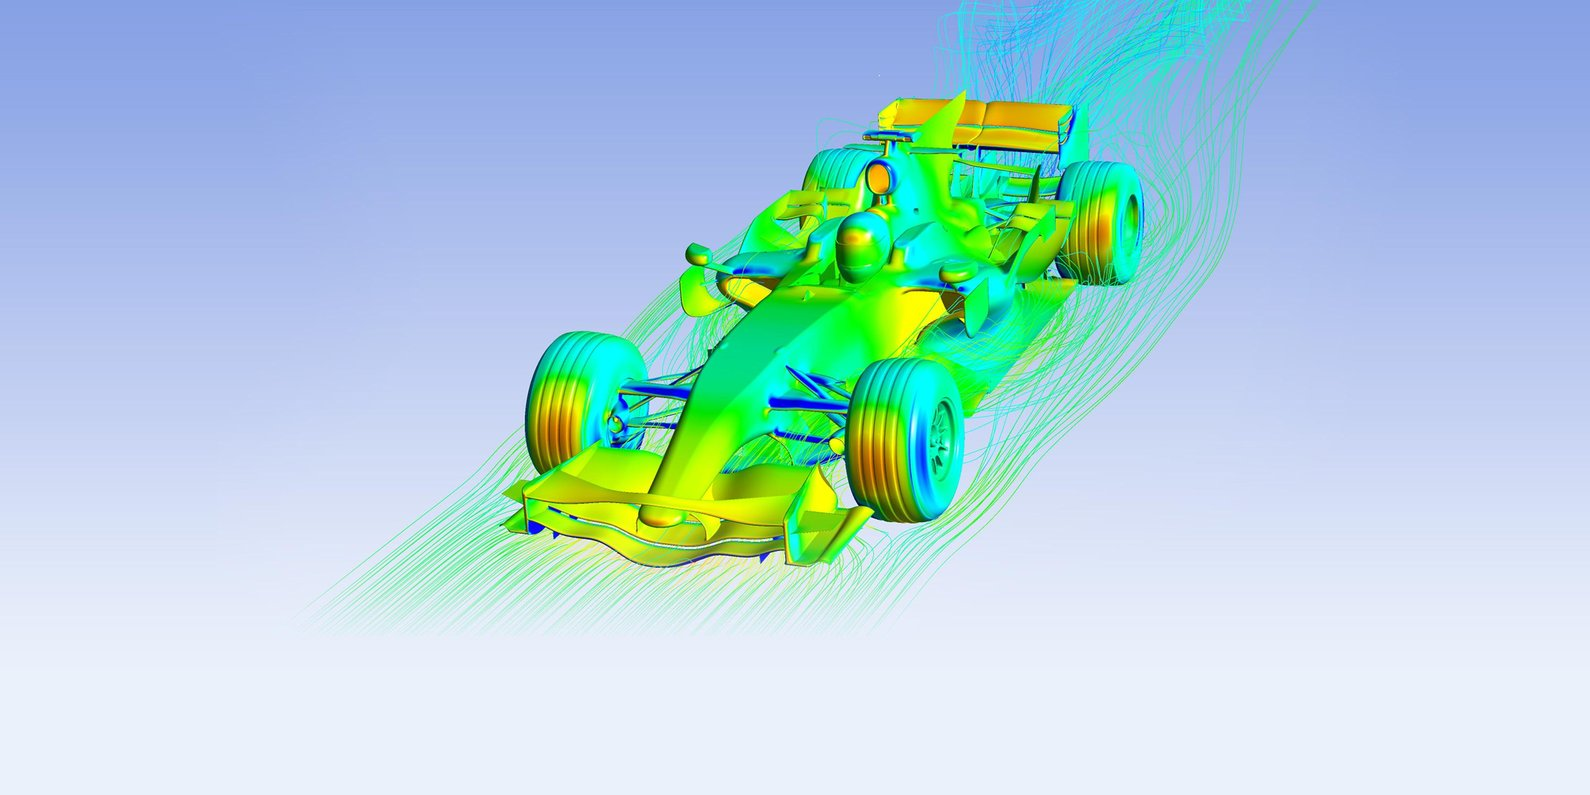
\includegraphics[width=.8\textwidth]{figs/cfd/redbull-ansys.jpg}
    \caption{Flow analysis over Red Bull Racing's F1 car.}
  \end{figure}
  {\small http://www.redbullracing.com/article/ansys-innovation-partner}
\end{frame}

\begin{frame}
  \frametitle{Automotive Engineers}
  \begin{figure} \centering
    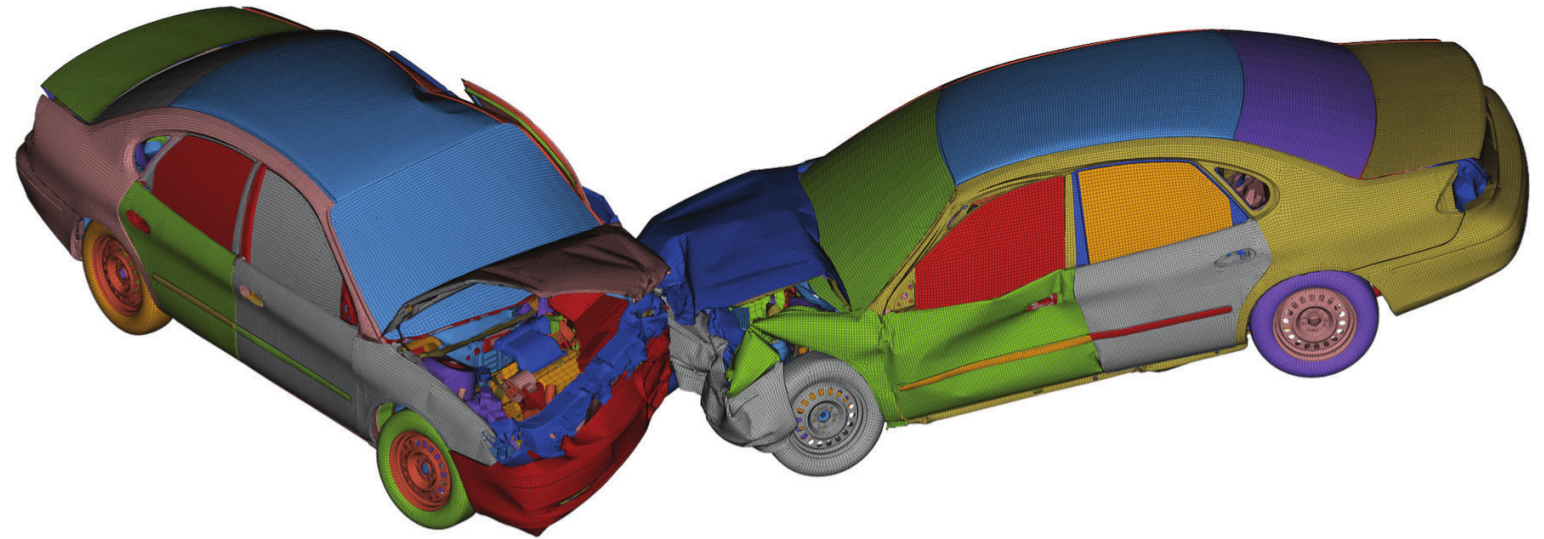
\includegraphics[width=.8\textwidth]{figs/cfd/altair-cray-crash-test.png}
    \caption{Optimizing High Fidelity Crash \& Safety Simulation Performance
  A Cray-Altair Solution for Manufacturing}
  \end{figure}
  {\small
    http://www.cray.com/sites/default/files/Altair-Cray-RADIOSS-Crash-Safety.pdf
  }
\end{frame}

\begin{frame}
  \frametitle{Biologists}
  \center Investment for creating one new drug is \$1B and 10 years 
  \center Novartis used HPC to screen 10M drugs in 11 hours for \$5k and 
          identified three compounds for further study
  \begin{figure} \centering
    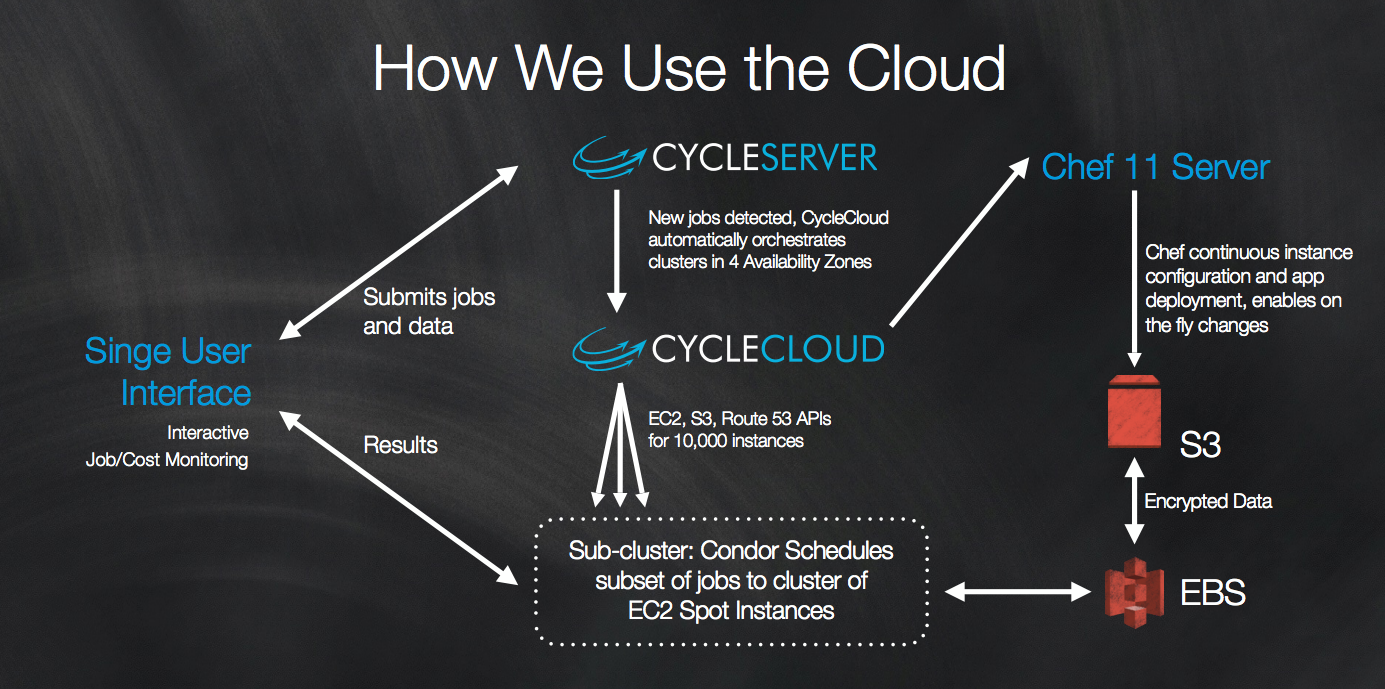
\includegraphics[width=.8\textwidth]{figs/bio/drug-discovery.png}
    \caption{\tiny http://cyclecomputing.com/blog/novartis-taps-cloud-hpc-for-faster-drug-discovery-better-science/ }
  \end{figure}
\end{frame}

\begin{frame}
  \frametitle{Chemists}
  \center 2013 Nobel Prize in Chemistry
  \center ``Their crucial achievement was to marry classical and quantum
   mechanics in order to model both the relatively large-scale movements of atoms
   in a molecule, and the minute dances of the free electrons that shuttle between
   atoms and spark many chemical reactions.''
   \begin{figure} \centering 
     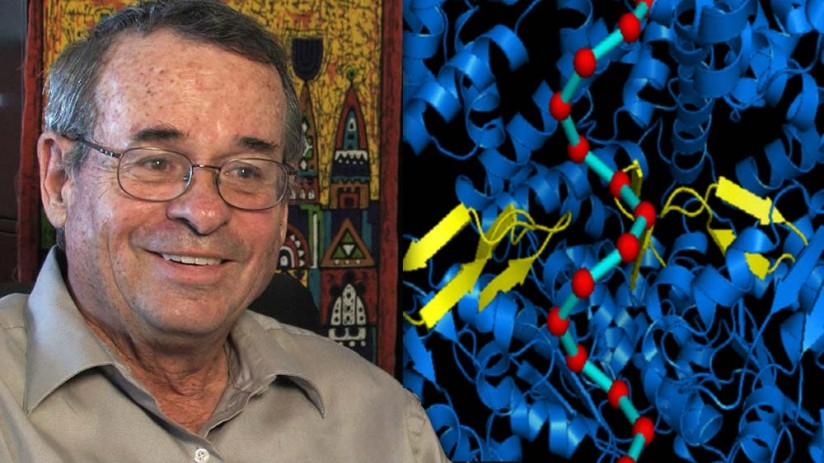
\includegraphics[width=.5\textwidth]{figs/chem/Warshel-2009-824x463.jpg}
     \caption{Arieh Warshel, Distinguished Professor of Chemistry at 
      USC Dornsife (USC Photo/Mira Zimet)}
   \end{figure}
   {\small http://news.usc.edu/56059/arieh-warshel-wins-nobel-prize/}
\end{frame}

\begin{frame}
  \frametitle{Physicists}
  \center Higgs Boson
  \center 90,000 processors at CERN to process massive amounts of data 
  \center 1,000,000,000,000,000 bytes per year
   \begin{figure} \centering 
     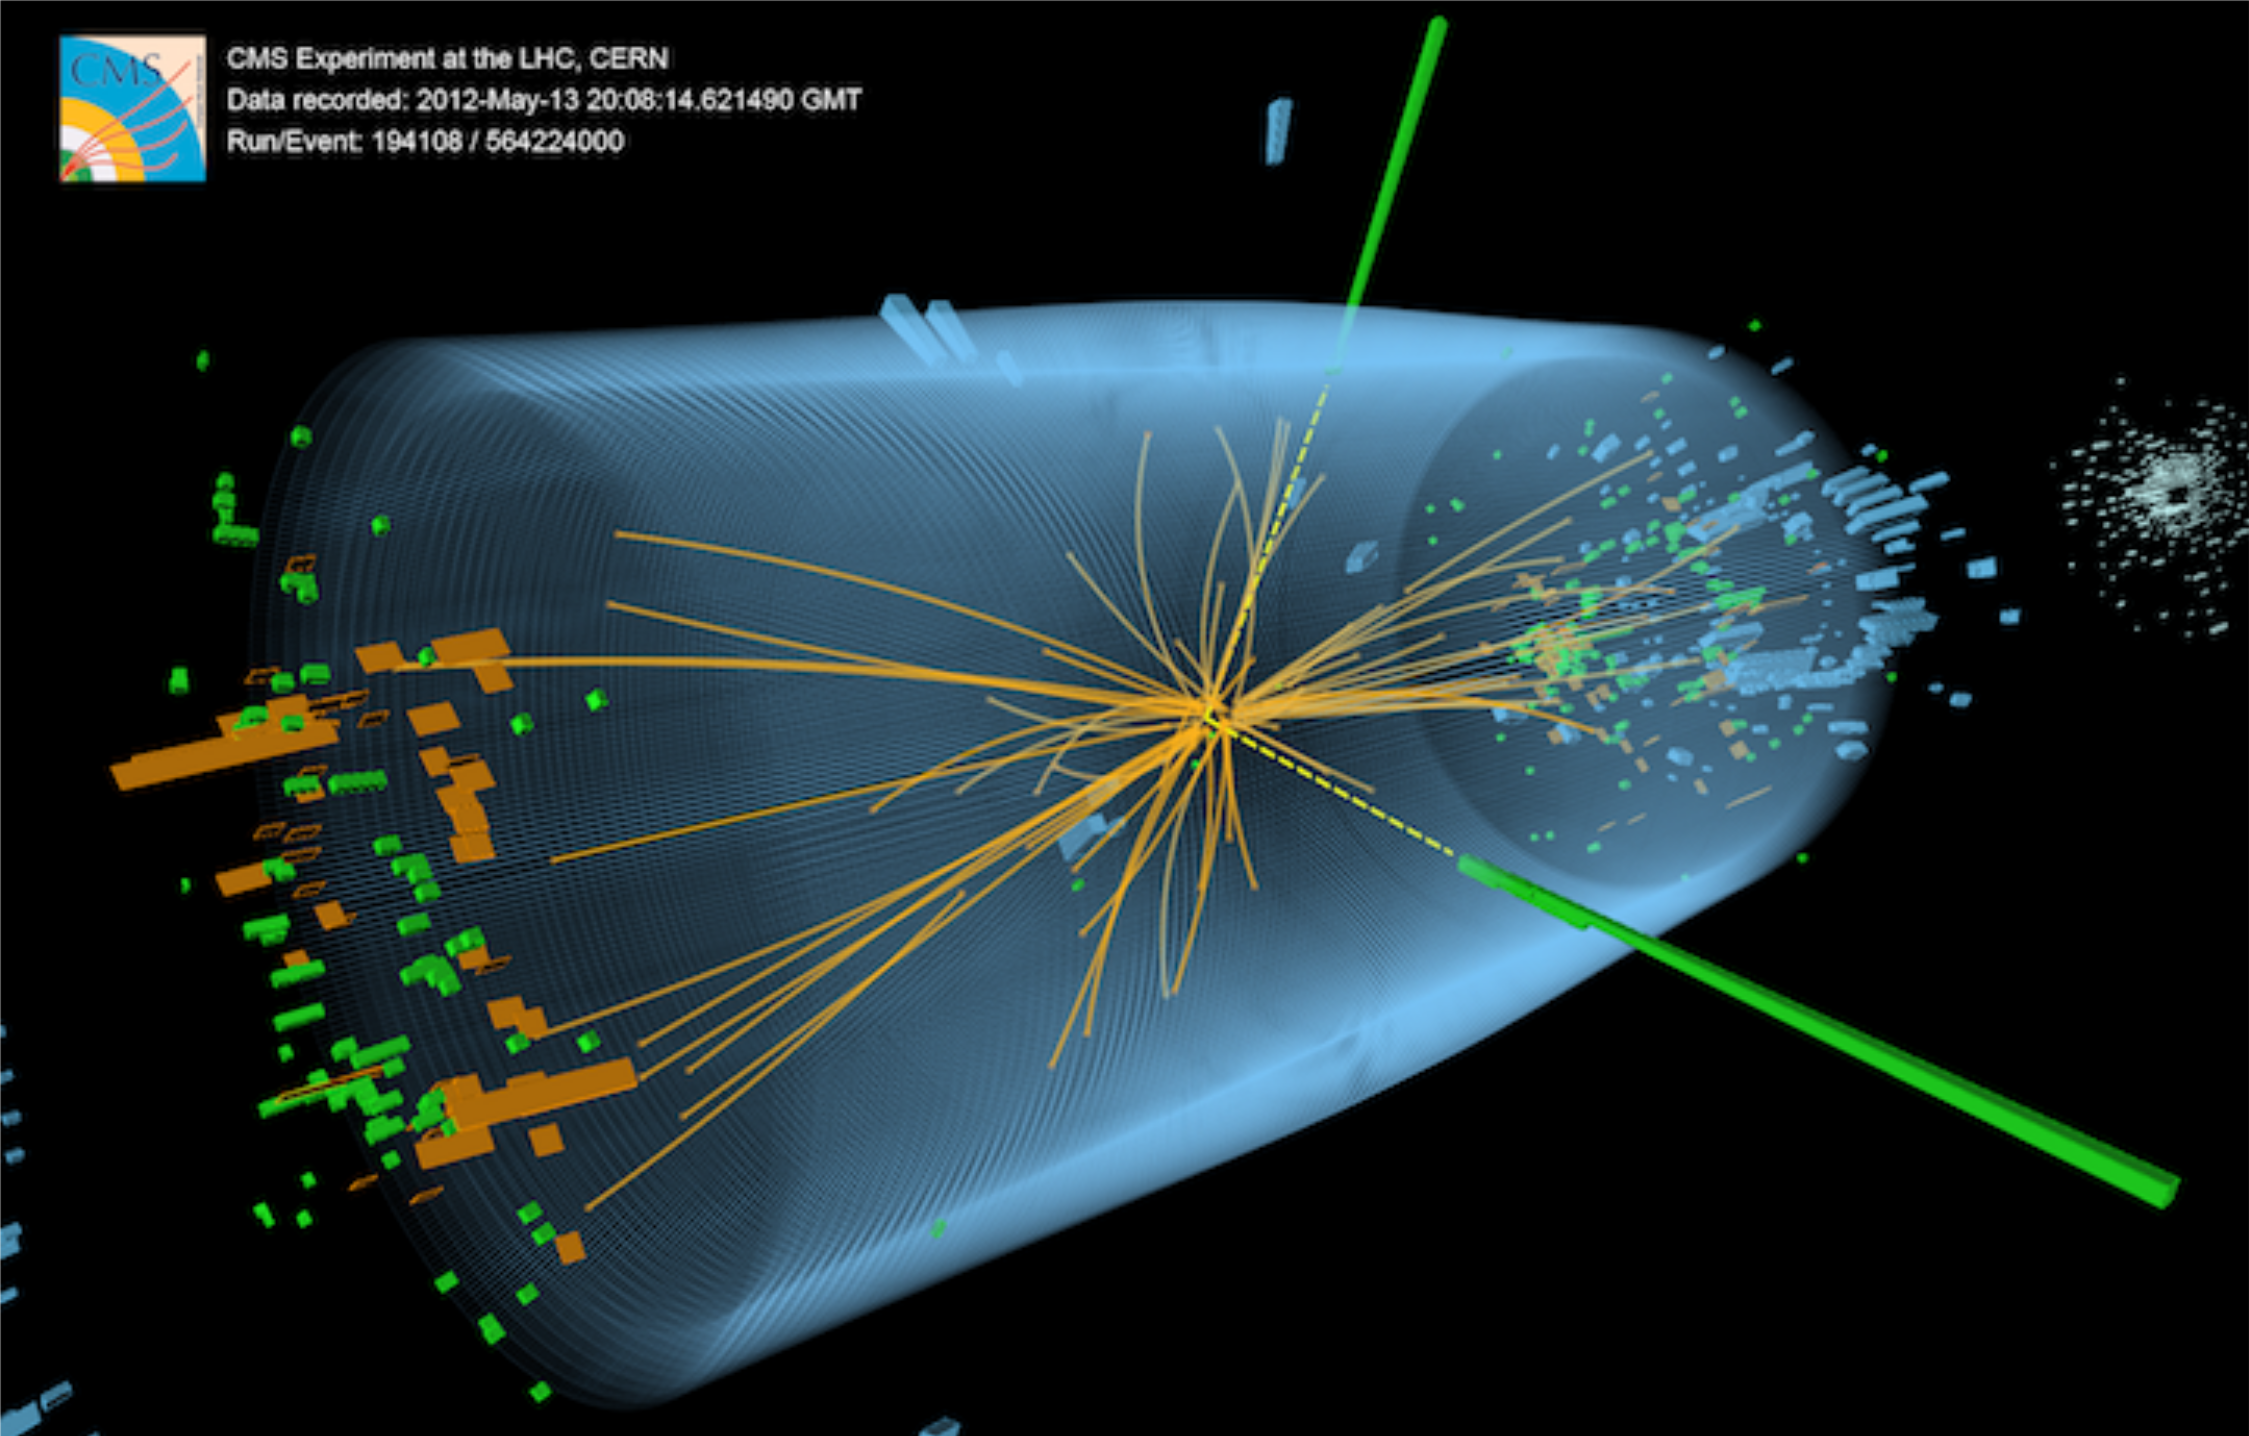
\includegraphics[width=.7\textwidth]{figs/phys/Candidate_Higgs_Events_in_ATLAS_and_CMS_cropped.png}
   \end{figure}
   {\small http://www.intel.com/content/www/us/en/high-performance-computing/high-performance-computing-xeon-e5-cern-higgs-boson-study.html }
\end{frame}

\begin{frame}
  \frametitle{Cryptologists}
  \center ``Today, all of the machines dedicated to mining Bitcoin have a
  computing power about 58,600 times the capacity of the United States
  government’s [second] mightiest supercomputer, the IBM Sequoia,'' says
  Taylor. \\
   \begin{figure} \centering 
     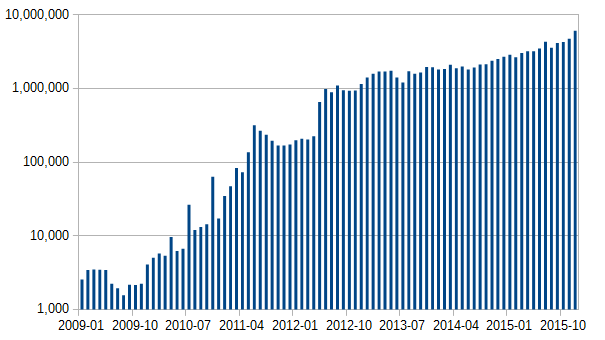
\includegraphics[width=.7\textwidth]{figs/crypt/BTC_number_of_transactions_per_month.png}
     \caption{Number of BTC transactions per month.}
   \end{figure}
  {\small http://www.hpcwire.com/2014/06/09/us-researcher-caught-mining-bitcoins-nsf-iron/ }
\end{frame}

\begin{frame}
  \frametitle{Computer Scientists}
  \center Computer Vision
  \begin{figure} \centering 
    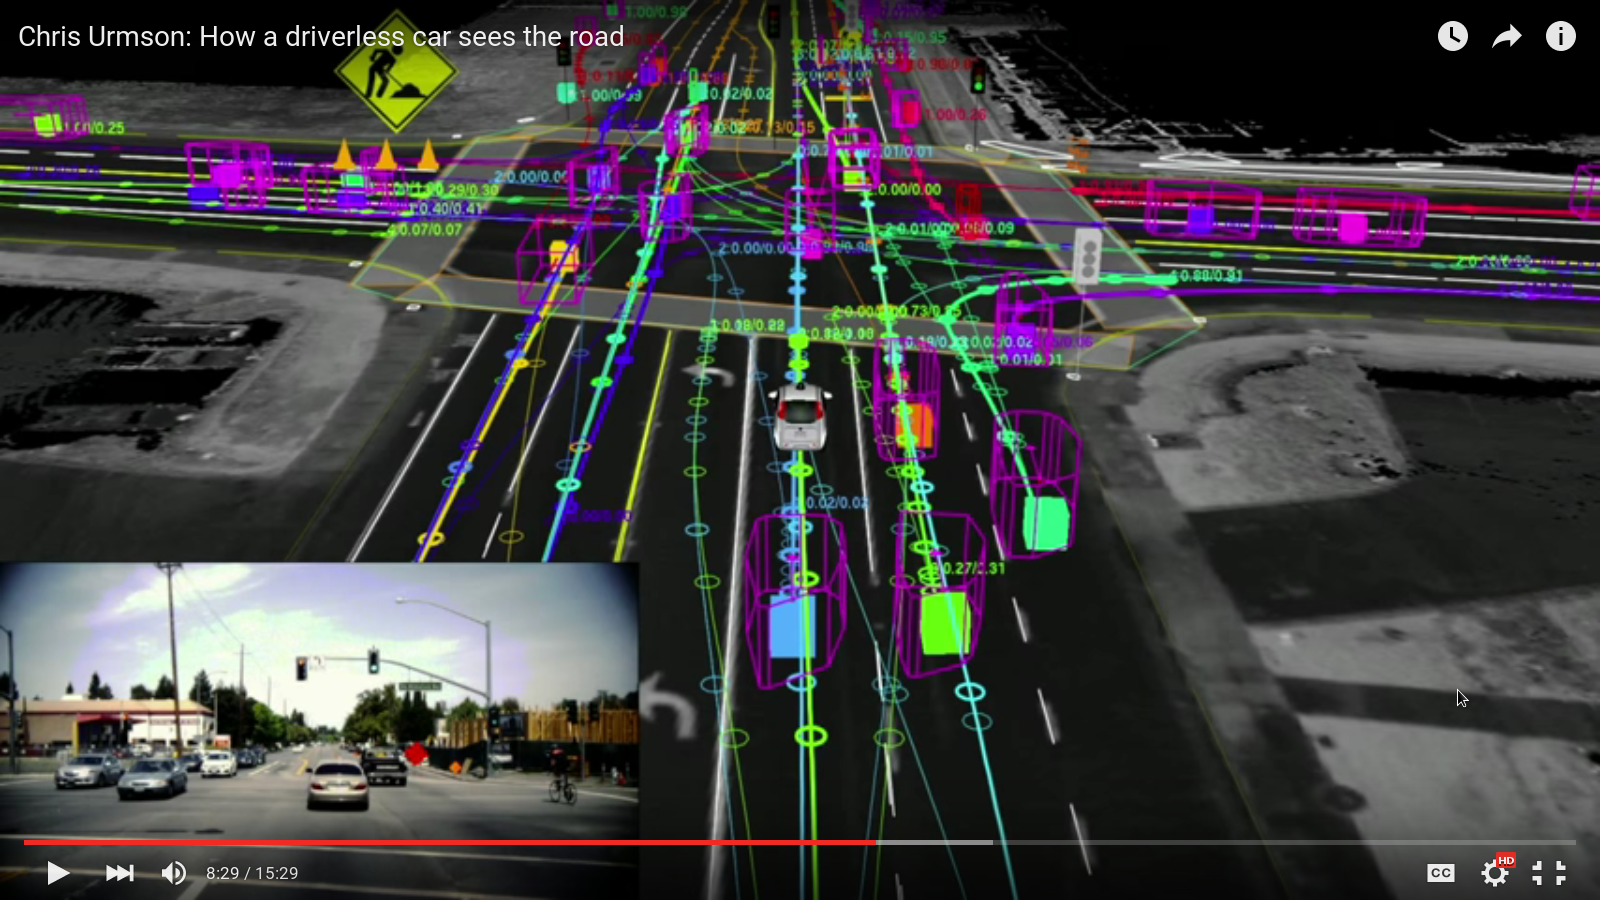
\includegraphics[width=.8\textwidth]{figs/compsci/google-comp-vision.png}
    \caption{Google TED Talk on Self Driving Cars}
  \end{figure}
  {\small https://www.youtube.com/watch?v=tiwVMrTLUWg}
\end{frame}

\begin{frame}
  \frametitle{Quantitative Analyst}
  \center High Frequency Trading
  \center ``These systems play the market without the guidance
  of humans; therefore they are only as good as their algorithms, which are
  generally kept as internal secrets within the respective firms. These
  supercomputers can be programmed to pursue any number or variation of
  strategies.''
  {\small http://www.qfac.ca/high-frequency-trading-an-evolving-exchange/ }
  \begin{columns}
    \begin{column}{0.5\textwidth}
      \begin{figure} \centering
	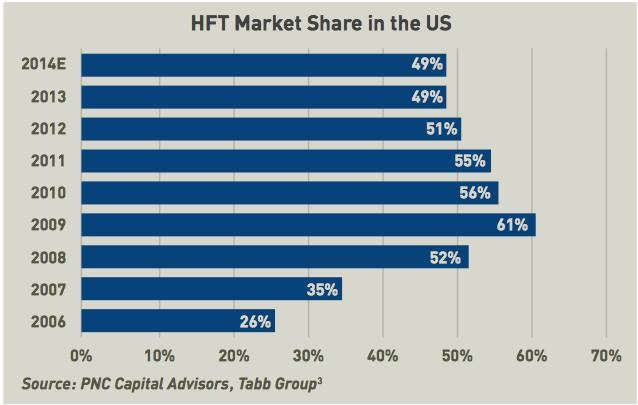
\includegraphics[width=.9\textwidth]{figs/hft/market-share.jpg}
      \end{figure}
    \end{column}
    \begin{column}{0.5\textwidth}
      \begin{figure} \centering
	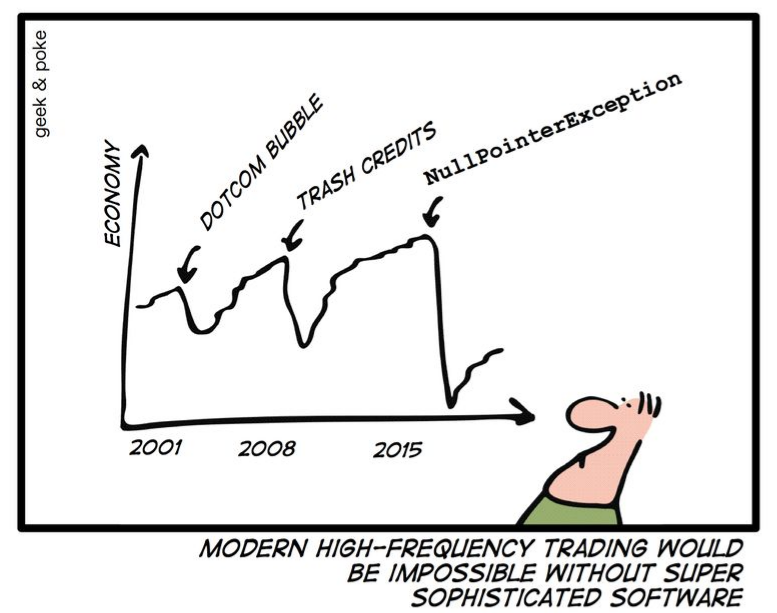
\includegraphics[width=.9\textwidth]{figs/hft/trading.png}
      \end{figure}
    \end{column}
  \end{columns}
\end{frame}


\begin{frame}
  \frametitle{Astronomers}
  \center Detecting Gravitational Waves
  \center ...``50 million core hours total to extract the signal and pull the
    science out of the data stream. We use a highly distributed computing
    environment with approximately 20,000 cores''
  \begin{figure} \centering 
    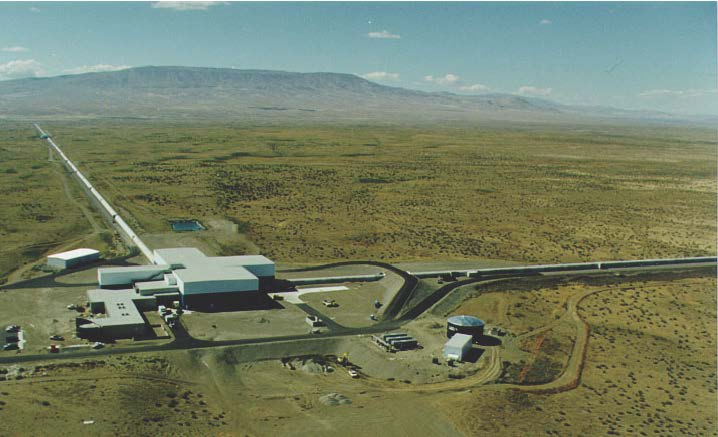
\includegraphics[width=.5\textwidth]{figs/ast/ligo.jpg}
    \caption{ \small LIGO Livingston Observatory in Louisiana.  Credit: MIT/CalTech LIGO }
  \end{figure}
  {\small http://www.scientificcomputing.com/articles/2016/03/hpc-helps-light-dark-universe-gravitational-wave-breakthrough }
\end{frame}

\begin{frame}
  \frametitle{Doctors}
  \begin{figure} \centering 
    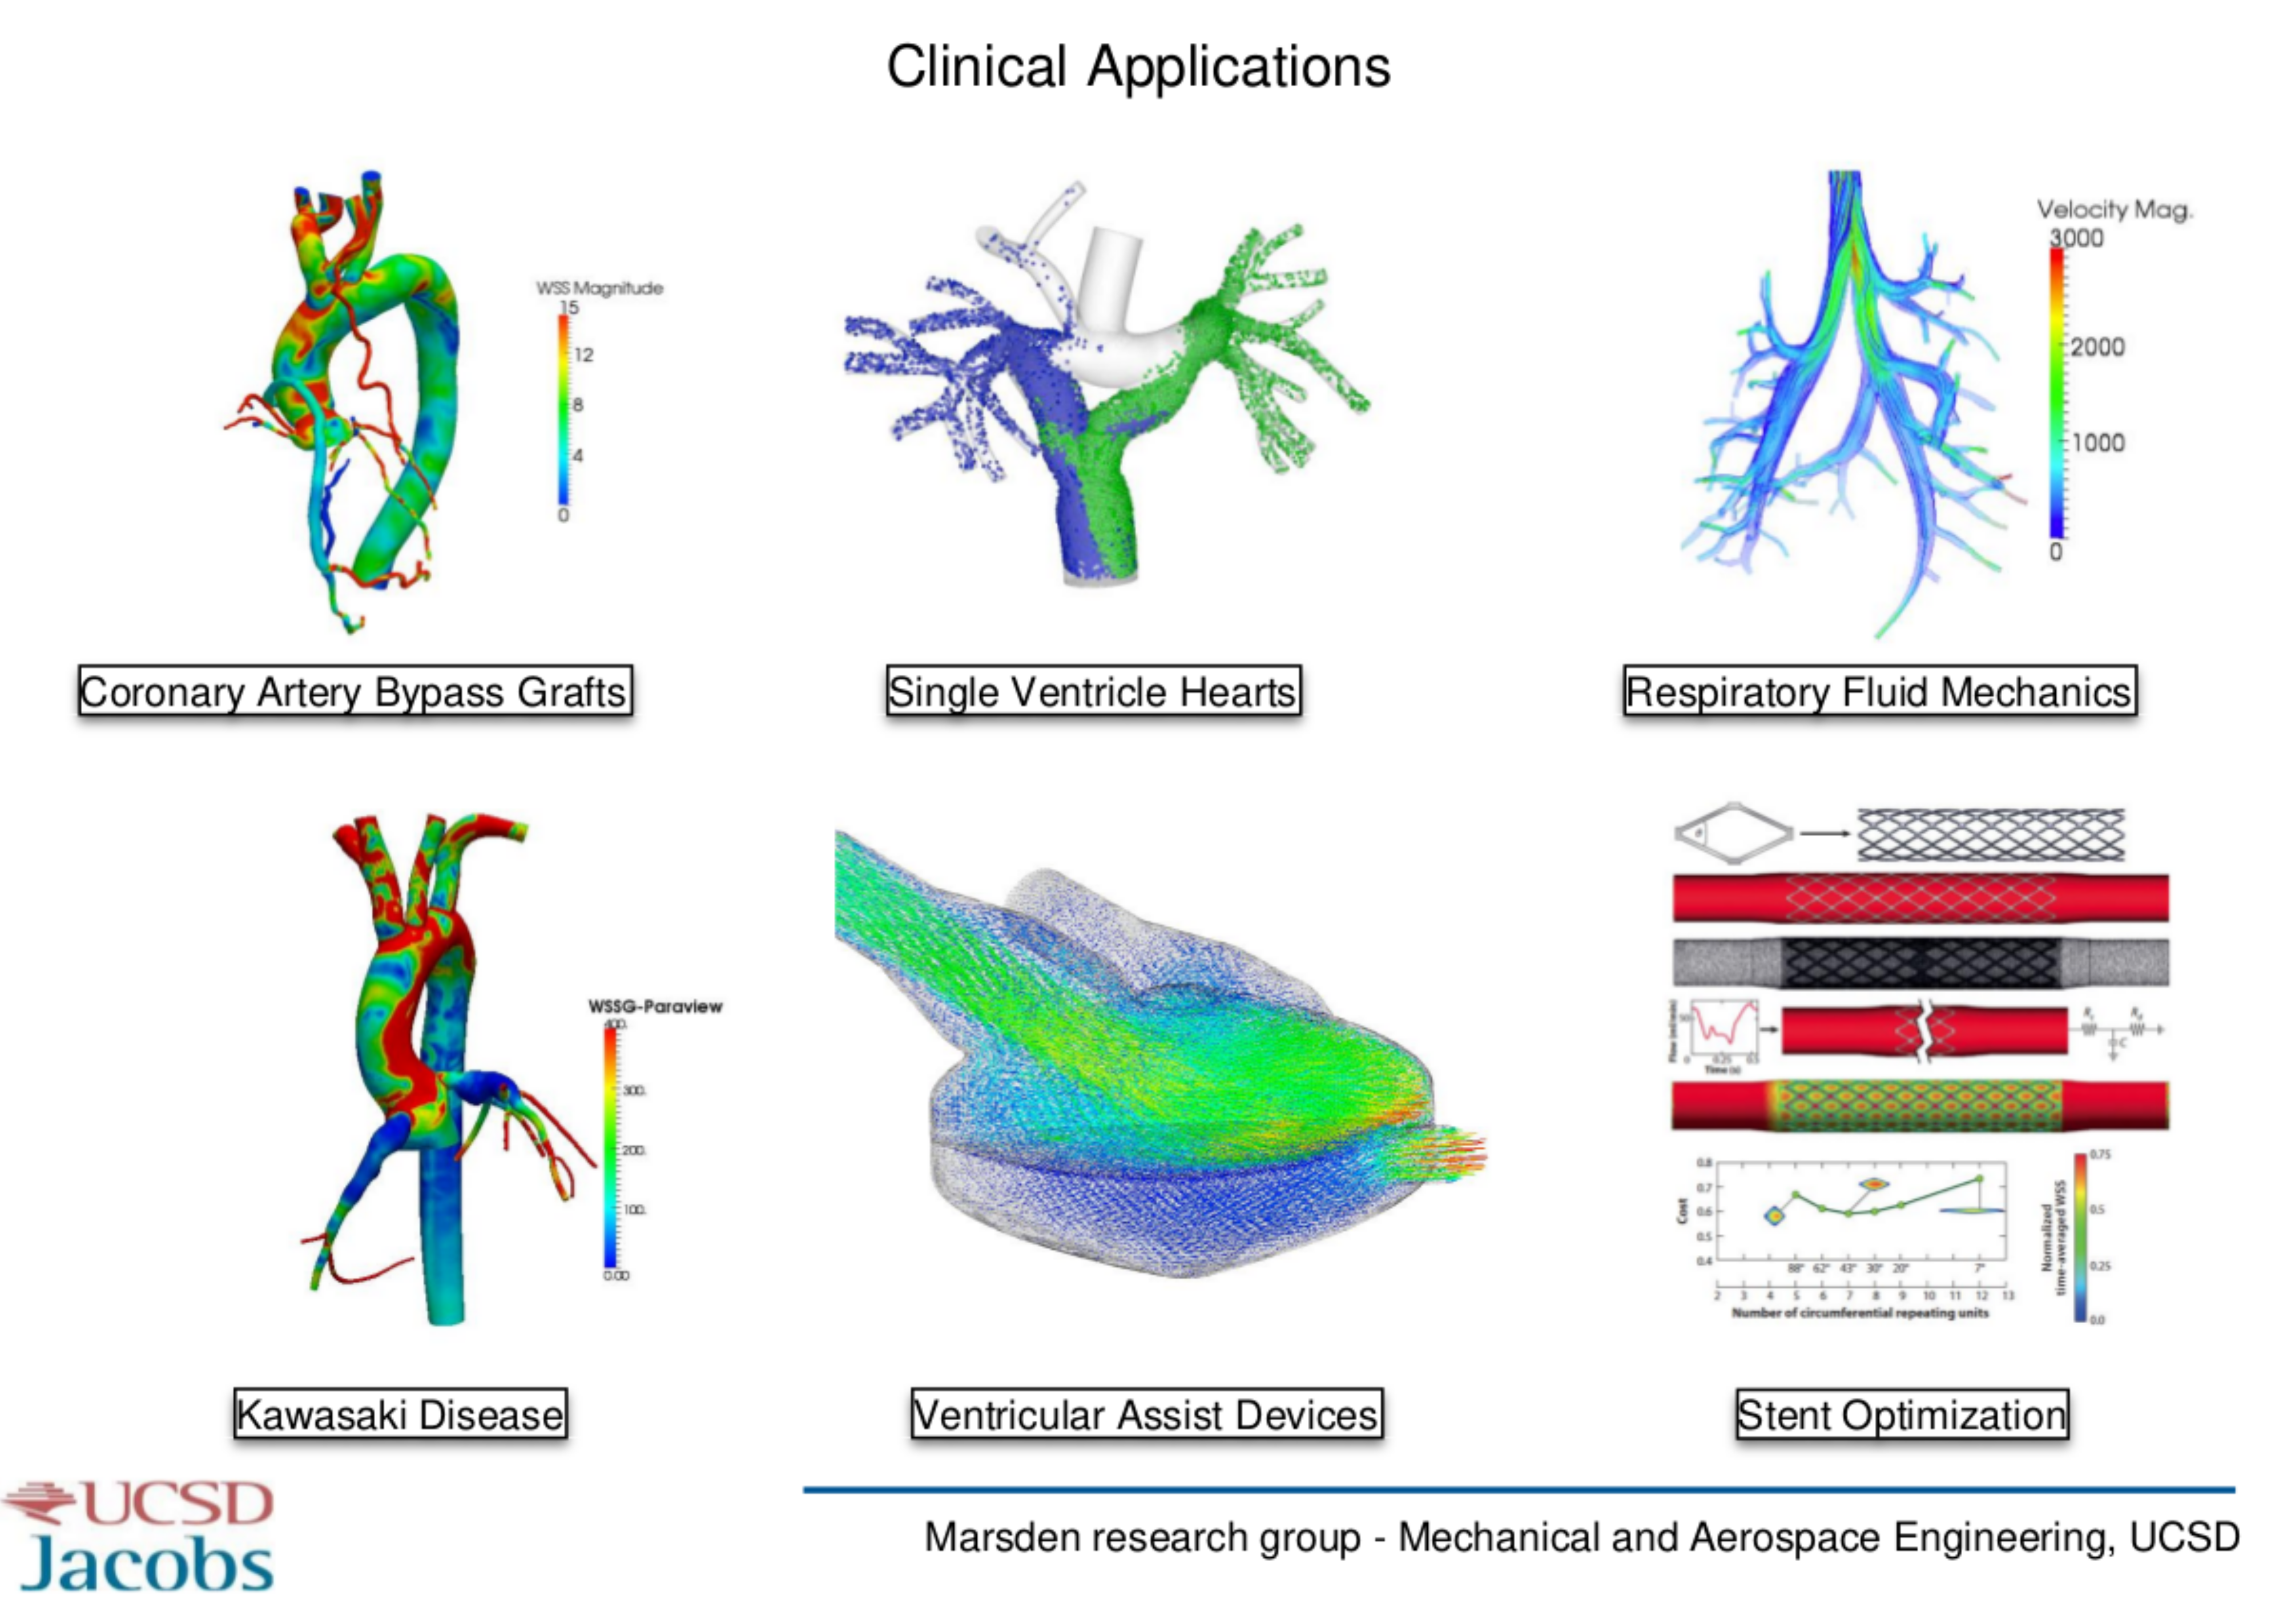
\includegraphics[width=.8\textwidth]{figs/doc/clinical-applications.png}
    \caption{Sim Vascular Software for Surgery Planning}
  \end{figure}
  {\tiny 
    http://idash.ucsd.edu/sites/default/files/uploads/08152014Marsden.pdf
  }
\end{frame}

\begin{frame}
  \frametitle{How to train yourself}
  \center Pick a domain.
  \center Learn it.
  \center Talk to people about it.
  \center Write about it.
  \center Read and write code for it.
\end{frame}

\begin{frame}
  \center Lots of code!
\end{frame}

\begin{frame}
  \frametitle{Our work}
  \center Solving PDEs on Unstructured Meshes
   \begin{figure} \centering 
     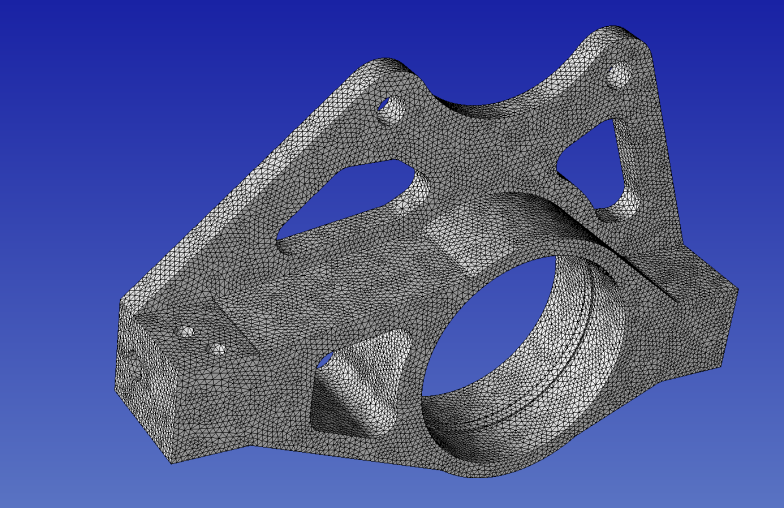
\includegraphics[width=.8\textwidth]{figs/mesh/upright.png}
     \caption{RPI Formula Hybrid Suspension Upright.}
  \end{figure}
\end{frame}

\begin{frame}
  \frametitle{My thesis work}
  \center Partitioning Unstructured Meshes
   \begin{figure} \centering 
     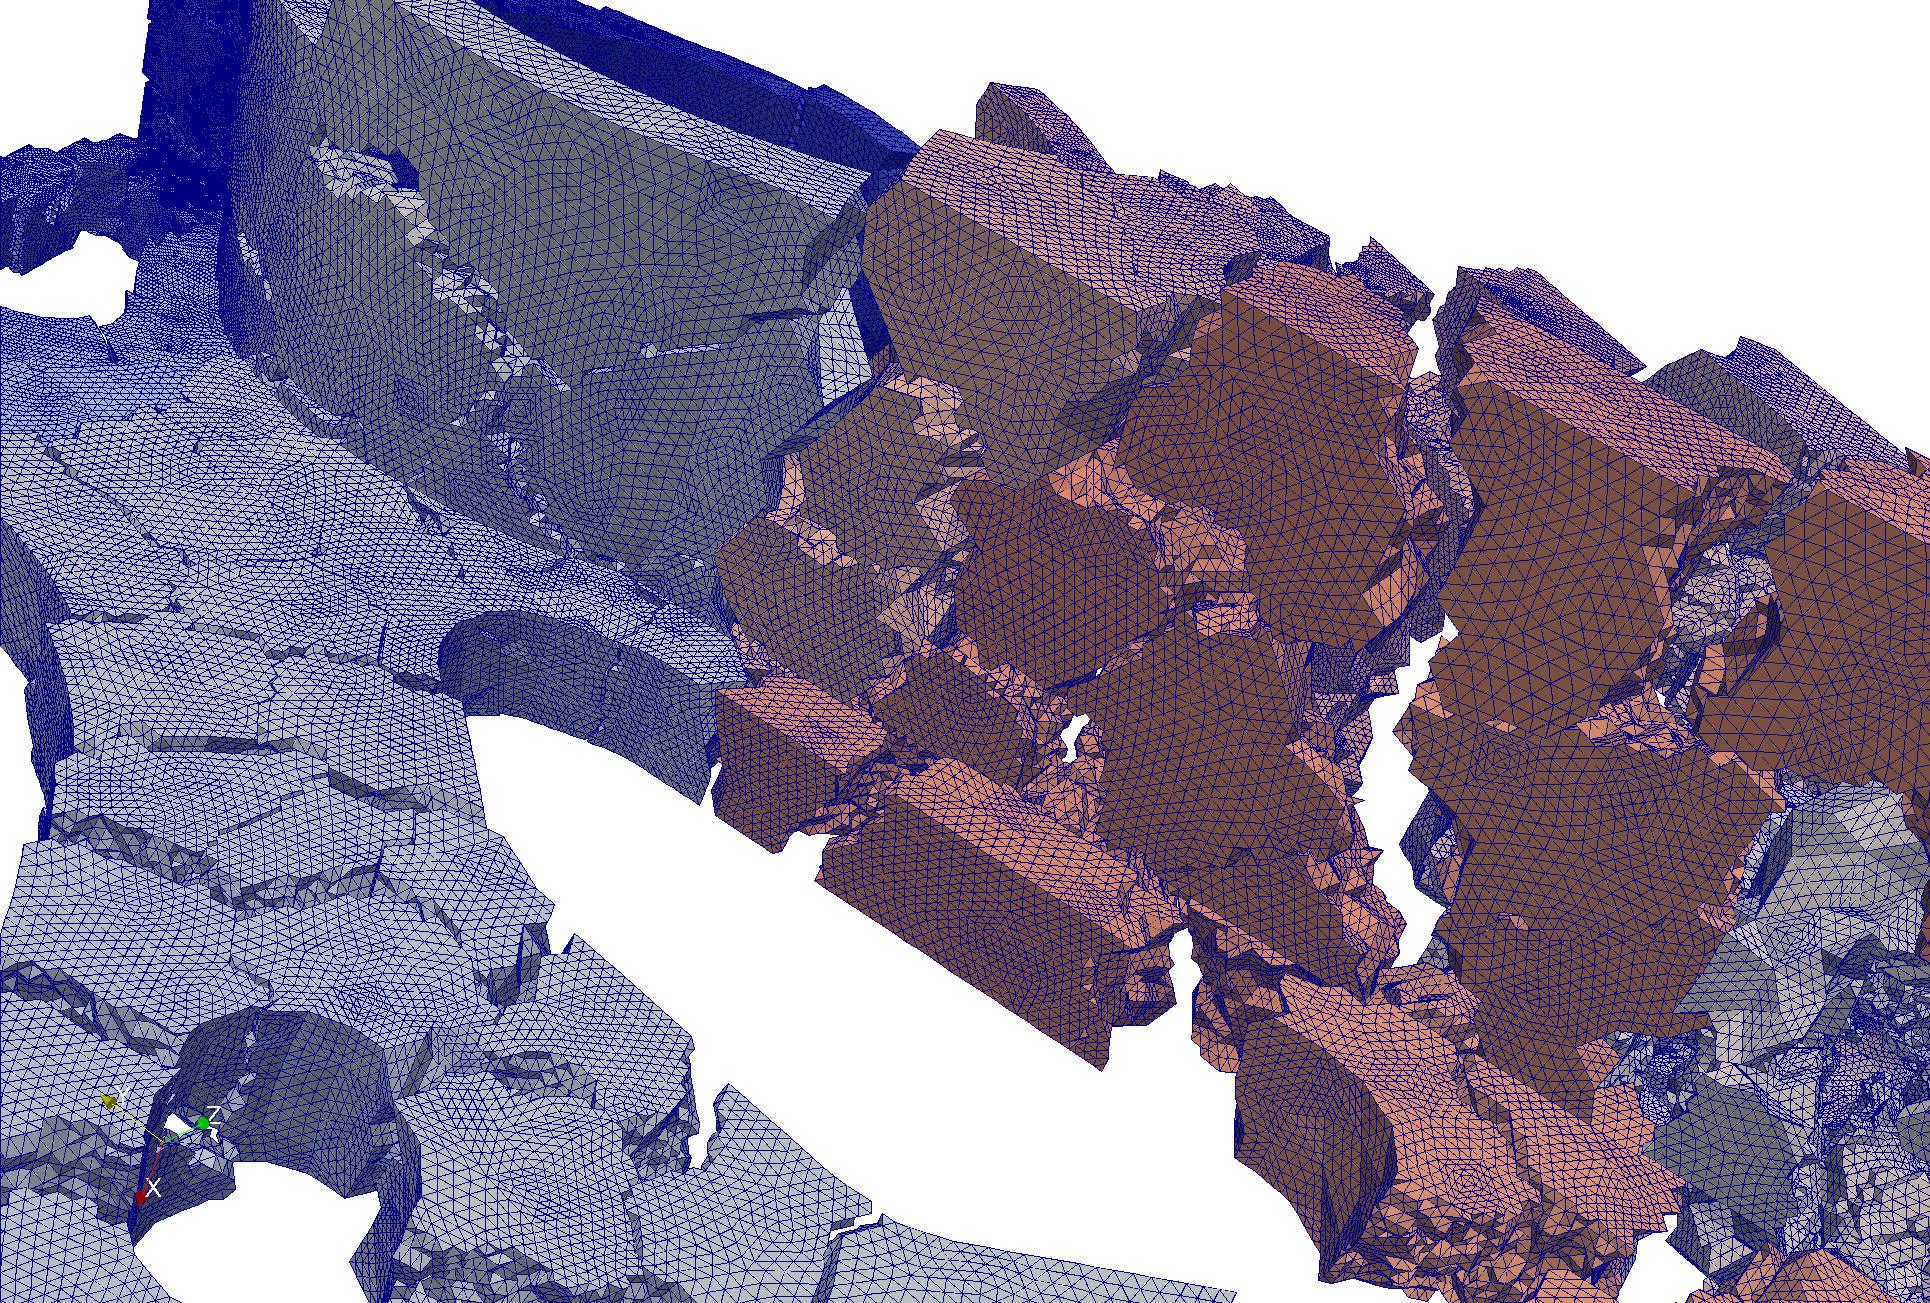
\includegraphics[width=.8\textwidth]{figs/mesh/upright512explodedWithEdgesZoom.png}
     \caption{A partitioned mesh.}
  \end{figure}
\end{frame}

\begin{frame}
  \center Thank You!
  \center Questions?
\end{frame}


\end{document}
